% Ensure that you compile using XeLaTeX !!! PDFTex has problems with some of the packages used
\documentclass[12pt]{article}
\setlength\parindent{0pt}

\usepackage{parskip}
\usepackage[margin=0.5in]{geometry}
\usepackage{fullpage}
\usepackage{moresize}
\usepackage{graphicx}
\usepackage{caption}
\usepackage{subcaption}
\usepackage{float}
\usepackage{xcolor}
\usepackage{soul}
\usepackage{fontspec}
\setmainfont{Doulos SIL}

\begin{document}

\begin{center}
\textbf{{\color{violet}{\HUGE 20201113 Friday\\}}}

\textbf{{\color{violet}{\HUGE ALL EXAMS (with notes)\\}}}

\end{center}
\newpage

\begin{center}
\textbf{{\color{blue}{\HUGE START OF EXAM\\}}}

\textbf{{\color{blue}{\HUGE Student ID: 45248\\}}}

\textbf{{\color{blue}{\HUGE 4:00\\}}}

\end{center}
\newpage

{\large Question 1}\\

Topic: Acoustics\\
Source: Week 9 Handout, Question 6\\

Explain what you see in the spectrogram that tells you about the properties of the sounds in the pictured word.\\

\begin{figure}[H]
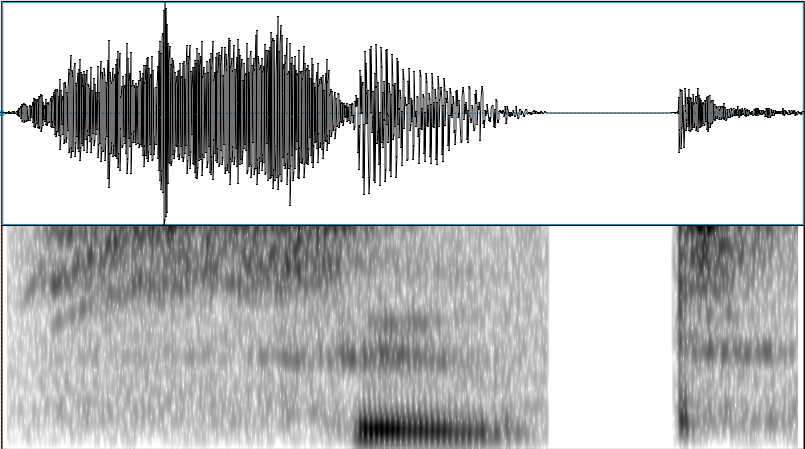
\includegraphics{../images/spectrogram_suit.png}
\end{figure}

~\\
INSTRUCTOR NOTES: suit: starts with fricative noise; then some kind of vowel; then a stop with a release burst; fricative is voiceless (no voice bar); fricative likely [s] because high-energy; vowel has low F1 (=high V) but then hard to see F2; stop is also voiceless


\vfill
Excellent (3) ~~~ Good (2.2) ~~~ Fair (1.7) ~~~ Poor (0)
\newpage

{\large Question 2}\\

Topic: Phonological Features\\
Source: Homework 2, Question 1\\

Explain which sound should be removed to make this a natural class (assuming SNAE, except that there are no diphthongs, no [ə] or [ʌ], no syllabic consonants, and no [w̥]), and what the minimum set of features would be to describe the resulting natural class.\\

{[i]}, {[ɪ]}, {[ɛ]}, {[u]}, {[ʊ]}


~\\
INSTRUCTOR NOTES: [ɛ] should be removed, so that we have the natural class of high vowels; this could be minimally represented with [+syll, +high]


\vfill
Excellent (3) ~~~ Good (2.2) ~~~ Fair (1.7) ~~~ Poor (0)
\newpage

\begin{center}
\textbf{{\color{red}{\HUGE END OF EXAM}}}\\

\end{center}
\newpage

\begin{center}
\textbf{{\color{blue}{\HUGE START OF EXAM\\}}}

\textbf{{\color{blue}{\HUGE Student ID: 99531\\}}}

\textbf{{\color{blue}{\HUGE 4:10\\}}}

\end{center}
\newpage

{\large Question 1}\\

Topic: Other (pre-midterm)\\
Source: Week 4 Handout, Part II, Question 2(iv)\\

Explain how you would figure out the Swahili word for this English gloss. (To be clear: you do NOT need to give me the Swahili form itself -- just explain the process of figuring it out.)\\

‘I wanted them.’

\begin{figure}[H]
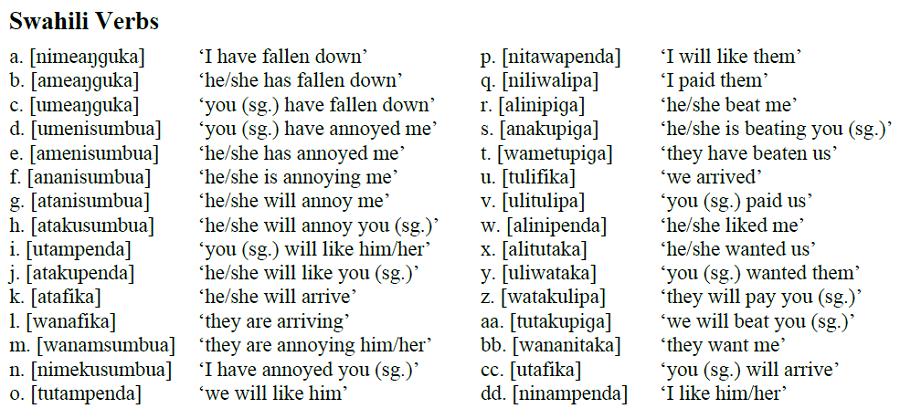
\includegraphics{../images/swahiliverbs.png}
\end{figure}

~\\
INSTRUCTOR NOTES: ([niliwataka])


\vfill
Excellent (3) ~~~ Good (2.2) ~~~ Fair (1.7) ~~~ Poor (0)
\newpage

{\large Question 2}\\

Topic: Articulatory Phonetics\\
Source: Week 3 Handout, Question 3\\

Explain why the additional vowel below either does or does not belong in the phonetic natural class defined by the original set of SNAE vowels.\\

Original set: {[ɛ]}, {[ɪ]}, {[ʊ]}, {[ɔ]}

Addition: {[æ]}


~\\
INSTRUCTOR NOTES: new vowel is a low vowel; should recognize that there's more than one decision about low vowels and tenseness; default is to say it doesn't belong in the class because tenseness is irrelevant


\vfill
Excellent (3) ~~~ Good (2.2) ~~~ Fair (1.7) ~~~ Poor (0)
\newpage

\begin{center}
\textbf{{\color{red}{\HUGE END OF EXAM}}}\\

\end{center}
\newpage

\begin{center}
\textbf{{\color{blue}{\HUGE START OF EXAM\\}}}

\textbf{{\color{blue}{\HUGE Student ID: 51191\\}}}

\textbf{{\color{blue}{\HUGE 4:20\\}}}

\end{center}
\newpage

{\large Question 1}\\

Topic: Phonological Features\\
Source: Week 4 Discussion\\

Explain what the given feature’s value is for this class of sounds, and why.\\

{[consonantal]}

glides


~\\
INSTRUCTOR NOTES: [-], because the constriction isn't as narrow as it would be for a fricative


\vfill
Excellent (3) ~~~ Good (2.2) ~~~ Fair (1.7) ~~~ Poor (0)
\newpage

{\large Question 2}\\

Topic: Articulatory Phonetics\\
Source: Homework 1, Question 3(a)\\

Could this image be the result of producing the sound represented by the given IPA symbol? Why or why not?\\

{[z]}

\begin{figure}[H]
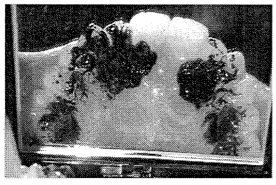
\includegraphics{../images/staticpalatography_fricative.png}
\end{figure}

~\\
INSTRUCTOR NOTES: yes


\vfill
Excellent (3) ~~~ Good (2.2) ~~~ Fair (1.7) ~~~ Poor (0)
\newpage

\begin{center}
\textbf{{\color{red}{\HUGE END OF EXAM}}}\\

\end{center}
\newpage

\begin{center}
\textbf{{\color{blue}{\HUGE START OF EXAM\\}}}

\textbf{{\color{blue}{\HUGE Student ID: 11925\\}}}

\textbf{{\color{blue}{\HUGE 4:30\\}}}

\end{center}
\newpage

{\large Question 1}\\

Topic: Acoustics\\
Source: Week 9 Handout, Question 5\\

Explain what would be similar and different about the sounds pictured and how you can tell from the pictures.\\

\begin{figure}[H]
\includegraphics{../images/vowel_spectra.png}
\end{figure}

~\\
INSTRUCTOR NOTES: SImilar: both are vowels, and in fact the same vowel quality, because the formants are in the same places. Different: the harmonics are differently spaced, so the fundamental frequency is different, and hence the pitches will be different. In particular, the top one has a LOWER pitch than the bottom one -- its harmonics are closer together, so the fundamental was a lower number to start with.


\vfill
Excellent (3) ~~~ Good (2.2) ~~~ Fair (1.7) ~~~ Poor (0)
\newpage

{\large Question 2}\\

Topic: Transcription\\
Source: Week 2 Handout, Part II, Question 11\\

How would this word be transcribed?\\ (Kathleen will then ask a follow-up question about your transcription.)\\

<juice>


~\\
INSTRUCTOR NOTES: [dʒus]


\vfill
Excellent (3) ~~~ Good (2.2) ~~~ Fair (1.7) ~~~ Poor (0)
\newpage

\begin{center}
\textbf{{\color{red}{\HUGE END OF EXAM}}}\\

\end{center}
\newpage

\begin{center}
\textbf{{\color{blue}{\HUGE START OF EXAM\\}}}

\textbf{{\color{blue}{\HUGE Student ID: 43736\\}}}

\textbf{{\color{blue}{\HUGE 4:40\\}}}

\end{center}
\newpage

{\large Question 1}\\

Topic: Skewed Distributions\\
Source: Week 5 Handout, Question 7\\

Explain how you would go about looking for co-occurrence restrictions in bi-syllabic signs in ASL. (Refer to the data that follows.)\\

\begin{figure}[H]
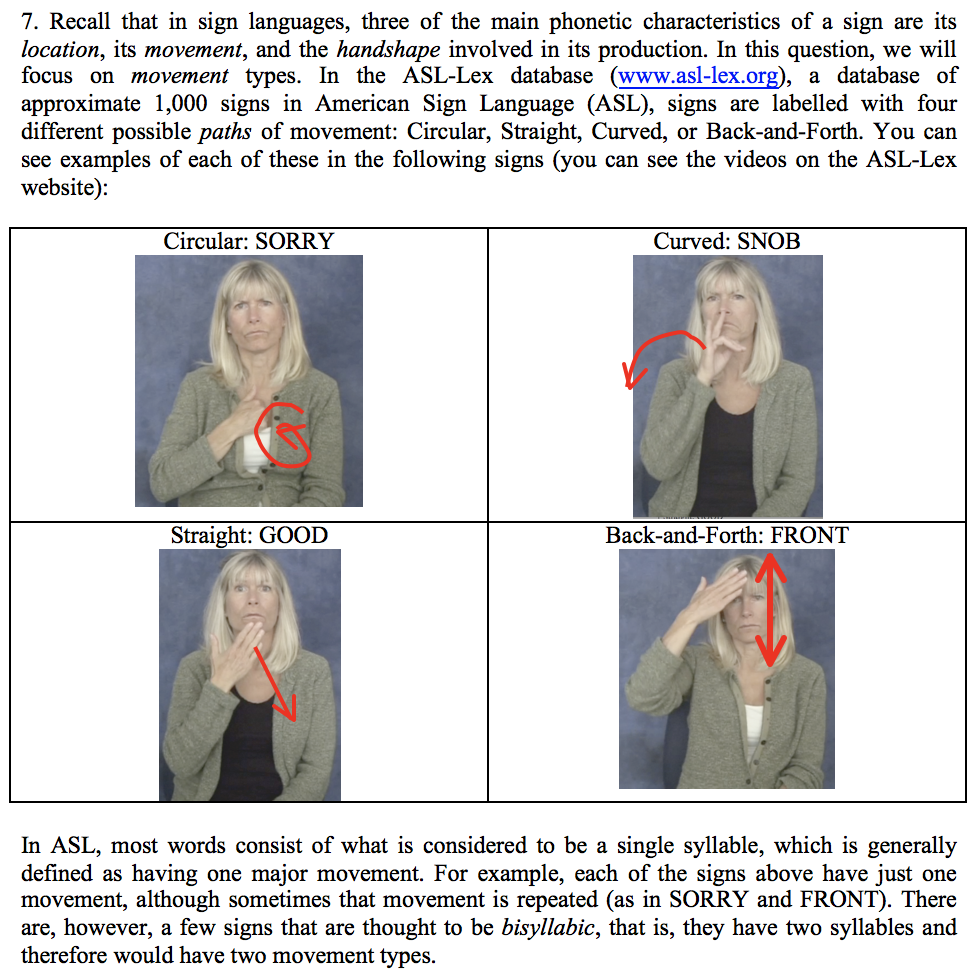
\includegraphics{../images/ASL_movement.png}
\end{figure}

~\\
INSTRUCTOR NOTES: You would start by coming up with all the possible combinations expected (i.e., 4x4 = 16). Then you'd compare that to some database of signs in ASL and see which combinations are actually attested or unattested.


\vfill
Excellent (3) ~~~ Good (2.2) ~~~ Fair (1.7) ~~~ Poor (0)
\newpage

{\large Question 2}\\

Topic: Articulatory Phonetics\\
Source: Week 3 Discussion\\

Assuming a Standard North American English inventory, does this vowel need to have tenseness specified if you're giving a prose description? Why or why not?\\

{[æ]}


~\\
INSTRUCTOR NOTES: no


\vfill
Excellent (3) ~~~ Good (2.2) ~~~ Fair (1.7) ~~~ Poor (0)
\newpage

\begin{center}
\textbf{{\color{red}{\HUGE END OF EXAM}}}\\

\end{center}
\newpage

\begin{center}
\textbf{{\color{blue}{\HUGE START OF EXAM\\}}}

\textbf{{\color{blue}{\HUGE Student ID: 74115\\}}}

\textbf{{\color{blue}{\HUGE 4:50\\}}}

\end{center}
\newpage

{\large Question 1}\\

Topic: Skewed Distributions\\
Source: Quiz 4, Question 1\\

L$_X$ (Language X) has three vowels, [i], [a], and [u]. It has bi-syllabic roots like Kikuyu. It does not allow non-identical high vowels to co-occur. Of the following nine logically possible vocalic sequences, which ones should be unattested in L$_X$? Explain why.\\

\begin{itemize} \item {[i...i]} \item {[i...a]} \item {[i...u]} \item {[a...i]} \item {[a...a]} \item {[a...u]} \item {[u...i]} \item {[u...a]} \item {[u...u]} \end{itemize}


~\\
INSTRUCTOR NOTES: [i...u], [u...i]


\vfill
Excellent (3) ~~~ Good (2.2) ~~~ Fair (1.7) ~~~ Poor (0)
\newpage

{\large Question 2}\\

Topic: Phonological Features\\
Source: Quiz 3, Question 12\\

Explain how you figure out which feature is involved in the process of umlaut shown below.\\

\begin{figure}[H]
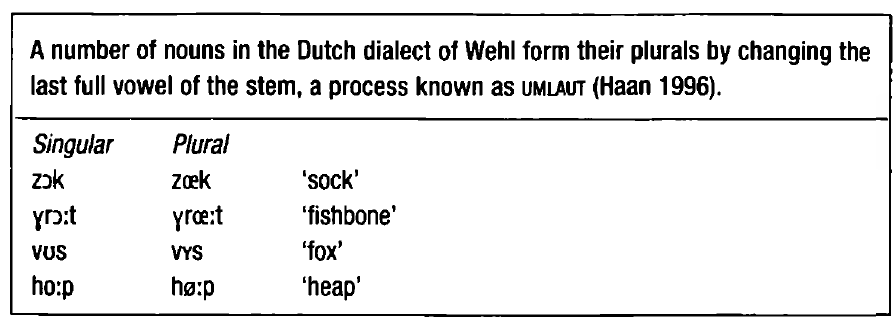
\includegraphics{../images/dutch.png}
\end{figure}

~\\
INSTRUCTOR NOTES: we look to see which vowels are affected, and compare them to see which feature is DIFFERENT (not e.g. what features they share); so since the vowels in the singular and plural are identical except that the singular forms are back and the plural are front, it's the feature [back] that is relevant / changing / involved (not e.g. the feature [round] just because all of the vowels are round)


\vfill
Excellent (3) ~~~ Good (2.2) ~~~ Fair (1.7) ~~~ Poor (0)
\newpage

\begin{center}
\textbf{{\color{red}{\HUGE END OF EXAM}}}\\

\end{center}
\newpage

\end{document}

